\documentclass[a4paper,10pt]{article}

% Packages
\usepackage[utf8]{inputenc}
\usepackage[frenchb]{babel}
\usepackage{graphicx}
\usepackage{url}
\usepackage{hyperref}
\usepackage{a4wide}
\usepackage{amsmath}
\usepackage{../../clrscode3epg}
%\usepackage{fullpage}
\renewcommand{\labelenumi}{(\alph{enumi})}

% Style
\parskip=\smallskipamount

% En-têtes
\title{
    \textbf{Structures de données et algorithmes}\\
    Projet 3: Analyse d'images
}

\author{Julien \textsc{Becker} - Gilles \textsc{Louppe} - Pierre \textsc{Geurts}}

\date{8 avril 2012}

% Corps
\begin{document}
\maketitle

\section*{\'Enoncé}

Ce projet vise à illustrer les techniques de résolution de problème et
les algorithmes de manipulation de graphes sur deux problèmes
d'analyse d'images. Nous vous demandons de remettre le code source
correspondant à votre implémentation ainsi qu'un bref rapport
répondant aux questions ci-dessous.

Le projet est à réaliser {\bf individuellement} pour le {\bf 18 avril
  2012} à {\bf 05h00} (du matin) au plus tard. Le projet est à
remettre via une interface web disponible sur
\href{http://www.montefiore.ulg.ac.be/~glouppe/2011-2012/students.info0902.php}{la
  page des TPs}.

Un projet non rendu à temps recevra automatiquement une cote nulle. En
cas de plagiat avéré, l'étudiant se verra affecter une cote nulle à
l'ensemble du projet. Les mêmes critères de correction que ceux
utilisés dans le cadre du cours
\href{http://www.montefiore.ulg.ac.be/~info0030/}{INFO0030 - Projet de
  programmation} seront utilisés pour évaluer l'implémentation des
algorithmes.

\subsection*{Fichier fourni}

Pour tester vos fonctions, nous vous fournissons:
\begin{itemize}
\item Une fonction \texttt{createImageFromFile} qui charge une image au format PGM et la stocke dans une structure \texttt{PortableGrayMap}.
\item Une fonction \texttt{saveImageToFile} qui prend en argument le nom de fichier et une structure \texttt{PortableGrayMap} et qui crée un fichier au nom fourni par l'utilisateur contenant l'image au format PGM.
\item Une fonction \texttt{createEmptyImage} qui permet de créer une image vide aux dimensions données.
\item Une fonction \texttt{deleteImage} qui permet de libérer la mémoire allouée à une image.
\end{itemize}

\subsection*{Fichiers à rendre}

Deux fichiers sont à rendre dans une archive \texttt{.tar.gz}. Le nom de l'archive n'a pas d'importance.
\begin{description}
\item[\texttt{ImageQuantizer.c}] implémente une fonction permettant de réduire le nombre de couleurs d'une image en 256 niveaux de gris à un nombre fourni par l'utilisateur
\item[\texttt{CountObjectsInImage.c}] implémente une fonction comptant les objets dans une image.
\item[\texttt{Rapport.pdf}] contient vos réponses aux questions
\end{description}

{\em Note}: Les noms de fichiers font partie de l'énoncé. Tout fichier ne
correspondant pas à ceux demandés dans l'énoncé ne sera pas pris en compte.

\section{Réduction des couleurs}

On souhaite écrire une fonction permettant de diminuer le nombre de
couleurs d'une image en $n$ niveaux de gris (par exemple $n=256$) vers
un nombre de niveaux $k$ inférieur (par exemple $k=8$). Cette
réduction entraînant immanquablement une perte de détails dans
l'image, l'objectif est de l'effectuer en préservant autant que
possible la qualité de l'image de départ. Un tel algorithme a beaucoup
d'applications telles que par exemple la compression d'image,
l'affichage d'une image sur un écran au nombre de couleurs limité ou
encore comme prétraitement pour permettre d'autres opérations
(identification de zones, etc.).

\subsection*{Formalisation du problème}

Soit l'image de départ représentée par une matrice $I$ de taille
$w\times h$ tel que $I[i,j]\in\{0,\ldots,n-1\}$ est le niveau du pixel
$(i,j)$. Le problème consiste à associer à chaque niveau $v\in
\{0,\ldots,n-1\}$ une nouvelle valeur parmi $k$ valeurs $\{v_1,
v_2,\ldots, v_k\} \subseteq \{0,\ldots, n-1\}$ telle que définie par une
fonction $g(v)$. On définira l'{\it erreur} associée à la réduction
comme la somme sur tous les pixels de l'image du carré de la
différence entre la valeur originale et la valeur compressée:
$$\sum_{i=1}^w\sum_{j=1}^h (I[i,j]-g(I[i,j]))^2,$$ où $g(.)$ est la
fonction qui associe à chaque niveau sa valeur ``compressée''.

Cette somme peut se réécrire en une somme sur tous les niveaux:
\begin{equation}\label{eqn:erreur}
\sum_{i=0}^{n-1} h[i] (i-g(i))^2,
\end{equation}
où $h[i]$, pour $i=0,\ldots,n-1$, est le nombre de pixels de l'image
de valeur $i$ (c'est-à-dire l'histogramme de l'image). L'objectif est
de déterminer la fonction $g$ et les valeurs $v_k$ qui minimise cette
erreur.

On peut montrer que le problème est équivalent à déterminer une
partition de $\{0,\ldots,n-1\}$ en $k$ sous-intervalles de valeurs
consécutives représentées chacunes par une même valeur, c'est-à-dire
considérer les fonctions $g$ de la forme:
\[
g(i)=\left\{
\begin{array}{ll}
v_1\mbox{ si }0\leq i<p_1\\
v_2\mbox{ si }p_1\leq i < p_2\\
\ldots\\
v_k\mbox{ si }p_{k-1}\leq i< n\\
\end{array}
\right.,
\]
où $0\leq p_1<p_2<\ldots<p_{k-1}<n$ et $v_1\leq v_2\leq\ldots \leq v_k$. Trouver la meilleure réduction revient
donc à déterminer les $k-1$ seuils $p_j$, $j=1,\ldots, k-1$ et les $k$
valeurs $v_j$, $j=1,\ldots,k$ de manière à minimiser l'erreur
(\ref{eqn:erreur}).


\paragraph{Exemple:} Soit l'image $5\times 5$
$$I=\left(\begin{matrix}
     3 & 6 & 0 & 4 & 0\\
     7 & 4 & 3 & 3 & 4\\
     4 & 1 & 1 & 0 & 0\\
     4 & 1 & 7 & 5 & 6\\
     6 & 7 & 5 & 0 & 6\\
\end{matrix}\right)
$$
en 8 valeurs de gris. Le vecteur du nombre de pixels par niveau est donné par:
$$h=[5,3,0,3,5,2,4,3].$$ Une représentation optimale en 3 niveaux est donnée par:
\[g(i)=\left\{
\begin{array}{ll}
1\mbox{ si }0\leq i<2\\
5\mbox{ si }2\leq i < 5\\
7\mbox{ si }5\leq i\leq 8\\
\end{array}
\right.,
\]
et son erreur est 11.

On vous demande d'implémenter les deux fonctions suivantes:
\begin{description}
%\item[] prenant comme argument une image et calculant le vecteur $f$ de fréquences des valeurs
\item[\texttt{computeOptimalReduction}] qui calcule les valeurs optimales de $p_1,\ldots,p_{k-1}$ et $v_1,\ldots,v_k$ à partir d'un vecteur de comptage $f$ et une valeur de $k$.
\item[\texttt{quantizeGrayImage}] qui réduit le nombre de niveaux de gris d'une image à un nombre $k$ de manière à minimiser l'erreur \ref{eqn:erreur}.
\end{description}

Une méthode de réduction du nombre de couleurs naïve qui ne tient pas
compte de l'erreur consiste à diviser l'intervalle $[0,n-1]$ en $k$
sous-intervalles de même taille et à associer à chaque sous-intervalle
la valeur centrale de l'intervalle. Cette variante est implémentée par
la fonction \texttt{quantizeGrayImageNaive} et vous est fournie pour
comparaison.

%% Nous vous fournissons une fonction ... uniforme qui calcule
%% l'intervalle de façon naïve en découpant de manière uniforme et en
%% associant à chaque sous-intervalle la valeur moyenne ...
%% $int( int(niveau/(n/k)) * (n/k))$

\subsection*{Suggestions}

Nous vous suggérons d'adopter la démarche suivante:
\begin{itemize}
\item Ecrivez une fonction permettant de calculer l'histogramme $h$ à
  partir d'une image
\item Pour un histogramme donné, déterminez (sur papier) le niveau de gris qui minimise l'erreur lorsqu'on réduit tous les niveaux entre $i$ et $j$ à ce même niveau et implémentez une fonction calculant cette valeur
\item Pour écrire la fonction \texttt{computeOptimalReduction}:
\begin{itemize}
\item Déterminez une formule de récurrence pour calculer l'erreur minimale résultant de la compression de $f$ en fonction de $n$ et de $k$;
\item Implémentez cette récurrence de manière efficace en utilisant le principe de programmation dynamique;
\item Modifiez votre implémentation pour calculer les valeurs des $p_i$ et $v_i$;
\item Améliorer éventuellement votre implémentation pour réduire les
  besoins en mémoire et accélérer les temps de calcul.
\end{itemize}
\end{itemize}

\subsection*{Questions}

Dans votre rapport:
\begin{itemize}
%\item Pourquoi est-ce que la méthode naïve n'est pas bonne ?
\item Expliquez la solution par programmation dynamique que vous avez implémentée
\item Comparer votre approche avec l'approche naïve sur l'image ...png fournie. Pourquoi est-ce que l'approche naïve ne fonctionne pas sur cette image ? Quand les deux approches sont-elles identiques ?
\item Analyser la complexité de la fonction \texttt{computeOptimalReduction} en fonction de $n$ et de $k$
%(Réponse: $\Theta(n^3 k)$ ou $\Theta(n^2 k)$ s'ils ont précalculé de manière intelligente les valeurs de $Err_{min}^1$)
%\item Complexité de l'approche force-brute en fonction de $n$ et de $k$ ?
%\item Comparer votre approche à celle implémentée par la fonction de compression naïve sur l'image ... fournie. Laquelle des deux approches est préférable ? Pourquoi ?
%  base (uniforme). Pourquoi cette approche est-elle préférable à
%  l'approche basique ?
%\item Bonus: si votre implémentation est $O(n^2 k)$.
%\item Bonus: expliquer pourquoi la formulation ... est en fait équivalente à la formulation
\end{itemize}

\section{Comptage d'objets au sein d'une image}

A partir d'une image contenant un certain nombre d'objets (représentés par des agglomérats de pixels claires sur un fond sombre), l'objectif est de compter le nombre d'objets
distincts dans l'image. Cette fonction peut par exemple être utilisée
pour compter le nombre d'étoiles dans des images astronomiques.

\subsection*{Formalisation du problème}

On travaillera ici sur des images de tailles quelconques $w\times h$
en 256 niveaux de gris et on représentera une image par une matrice
comme dans la première partie du projet. On définira les pixels
claires constitutifs des objets comme ceux dont l'intensité est
supérieure à un seuil $i_{th}$ (fourni par l'utilisateur ou calculé
automatiquement en appelant l'algorithme de réduction de couleur avec
$k=2$). Chacun des pixels clairs peut être considéré comme un sommet
d'un graphe non dirigé. Les sommets correspondant à deux pixels sont
connectés par un arc dans le graphe si les deux pixels sont voisins
dans l'image. On considèrera qu'un pixel de coordonnées $(x,y)$ est
voisin des 8 pixels de coordonnées $(x-1,y-1), (x,y-1), (x+1,y-1),
(x+1,y), (x+1, y+1), (x,y+1), (x-1,y+1), (x-1,y)$ (pour autant que
ceux-ci existent dans les limites de l'image).

Le problème du comptage d'objets revient alors à calculer le nombre de
composantes connexes dans le graphe.

\paragraph{Exemple:} Soit l'image $4\times 4$
$$I=\left(\begin{matrix}
170&220&110&250\\
100&10&230&215\\
210&90&60&150\\
230&80&120&40
\end{matrix}\right).
$$
En prenant un seuil $i_{th}=200$, le graphe des pixels clairs est donné par:
\begin{center}
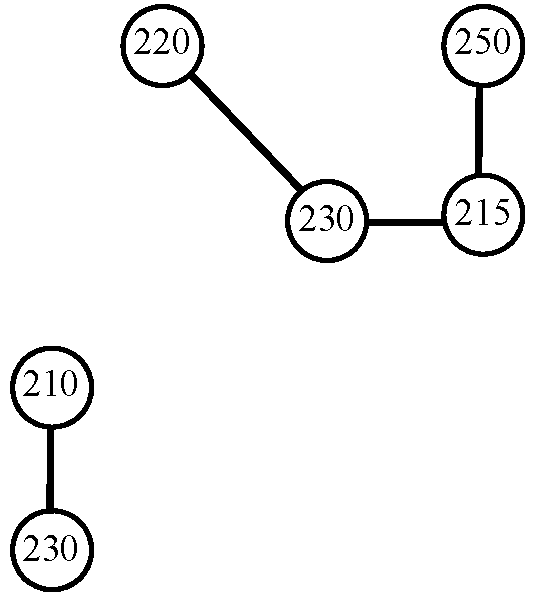
\includegraphics[width=4cm]{pict3.pdf}
\end{center}

On vous demande d'écrire une fonction \texttt{countObjectsInImage}
prenant en argument une image et un seuil $i_{th}$ et renvoyant le nombre d'objets
présents dans l'image.

\subsection*{Suggestions}

Nous vous suggérons d'adopter la démarche suivante:
\begin{itemize}
%\item Déterminer le seuil automatiquement en utilisant la fonction ... développée précédemment
\item Implémentez une fonction calculant le graphe des pixels clairs à partir de l'image et du seuil $i_{th}$
\item Ecrivez une fonction auxiliaire prenant en argument un graphe et calculant le nombre de composantes connexes.
\end{itemize}

\subsection*{Questions}

\begin{itemize}
\item Expliquez et motivez la solution que vous aurez adoptée
\item Analyser la complexité de votre implémentation d'abord en fonction de la
  taille du graphe extrait de l'image et ensuite en fonction de la taille de
  l'image.
\item Utilisez votre algorithme pour calculer le nombre d'étoiles dans
  l'image star.png fournie, après avoir déterminé le seuil $i_{th}$ en utilisant la fonction \texttt{quantizeGrayImage} avec $k=2$ ($i_{th}$ sera alors pris égal à $p_1$).
\end{itemize}


\end{document}
